Для выбора оптимального варианта реализации многорежимного формирователя импульсной последовательности необходимо задаться критерием, по которому можно было бы сравнить два описанных вариант, и выбрать один. В качестве данного критерия был выбран: минимум аппаратных затрат. \\
Для оценки аппаратных затрат была использована САПР Quartus, при помощи которой были скомпилированы оба варианта для целевой ПЛИС. Компиляция показала количество задействованных логических элементов.
\begin{figure}
  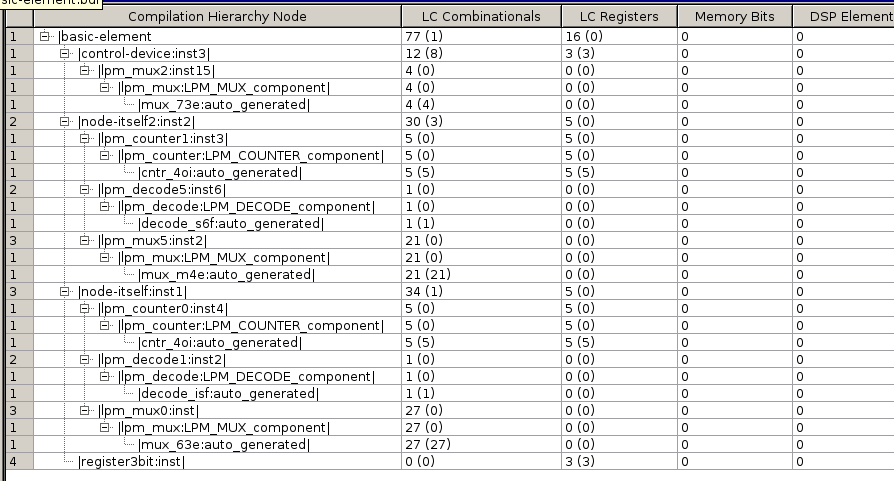
\includegraphics[scale=0.65]{./logics-count.png}
  \caption{Количество логических элементов, затраченных на реализацию обоих вариантов схемы на ПЛИС Cyclone II EP2C5Q208C8}
  \label{fig:logicscount}
\end{figure}
Из рисунка \ref{fig:logicscount} видно, что первый вариант схемы занимает на ПЛИС 34 логических элемента, второй вариант - 30. По выработанному нами критерию, выбираем второй вариант схемы.